\chapter{Apéndice: diseño de redes neuronales} \label{chapter:appendixA}
\begin{definition}[Normalización por lotes (\textit{Batch normalization})]
    Sea \( \mathcal{B} = (x_{i})_{i=1}^m \) con \( x_{i} \in \real{n} \) un minilote con media \( \widehat{\mu}_\mathcal{B} \) y desviación estándar  \( \widehat{\sigma}_\mathcal{B} \). Sean \( \gamma, \beta \in \real{n} \).

    Definimos la normalización por lotes como la capa que computa la función \( \BN: \real{n} \to \real{n} \):
    \[
        \BN(x; \gamma, \beta) = \gamma \odot \frac{x - \widehat{\mu}_\mathcal{B}}{\widehat{\sigma}_\mathcal{B}} + \beta
    \]
\end{definition}

La normalización por lotes funciona bien cuando el tamaño de cada minilote es suficientemente grande como para que los estimadores \( \widehat{\mu}_\mathcal{B}, \widehat{\sigma}_\mathcal{B} \) sean próximos al valor poblacional (lo que requiere, por lo general, un tamaño de minilote de entre 50 y 100 elementos \cite{luo2018towards}).

\begin{figure}[tb]
    \centering
    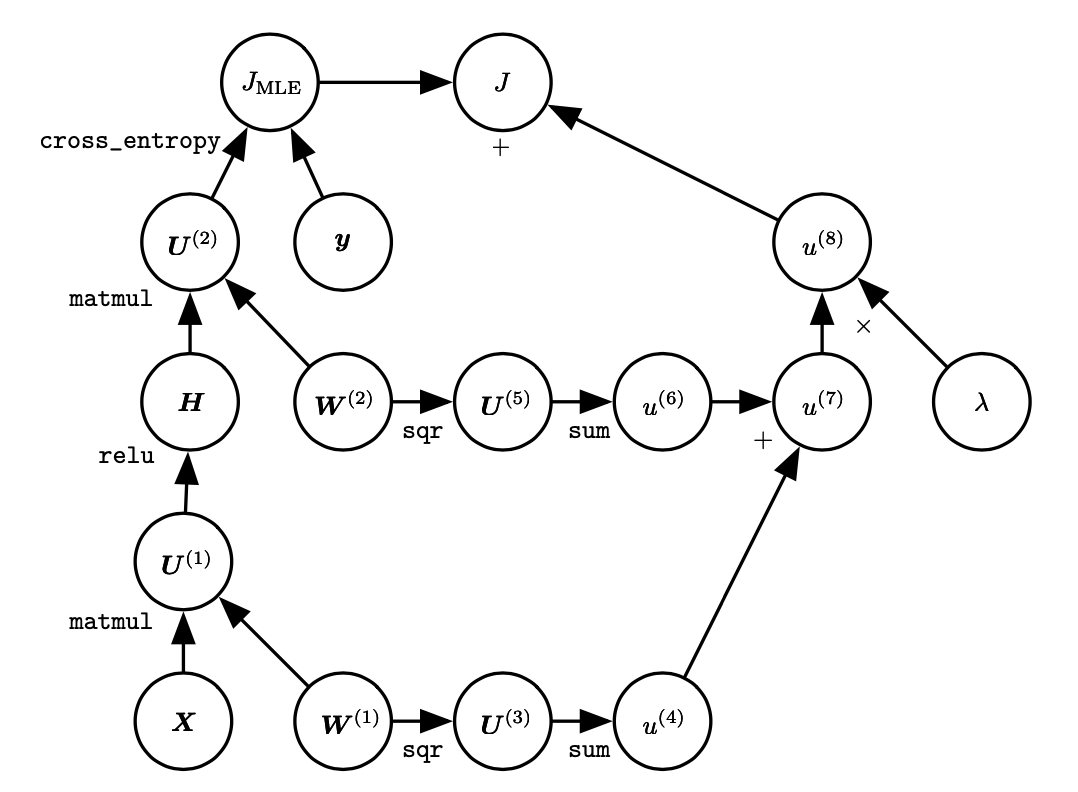
\includegraphics[scale=0.6]{figures/chapter2/grafo.png}
    \caption{Ejemplo de grafo computacional de una red sencilla. El grafo se construye durante la propagación hacia delante en el sentido de las aristas y el gradiente se calcula durante la propagación hacia atrás en sentido inverso, comenzando por la pérdida (nodo \( J\)) \cite{goodfellow2016deep}}
    \label{fig:graph}
\end{figure}


\begin{figure}[tb]
    \centering
    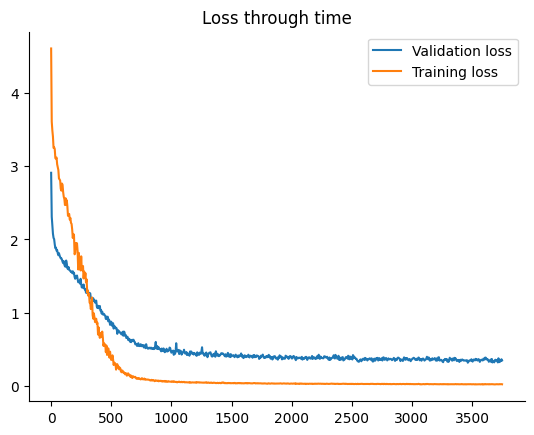
\includegraphics[scale=0.5]{figures/chapter5/loss_big.png}
    \caption{Pérdida sobre el conjunto de entrenamiento y validación a lo largo del entrenamiento. Los valores no son comparables con los de la \cref{fig:loss}, pues la división en símbolos se hace ahora a nivel de palabra, no de caracter. }
    \label{fig:loss_big}
\end{figure}
\begin{figure}[tb]
    \centering
    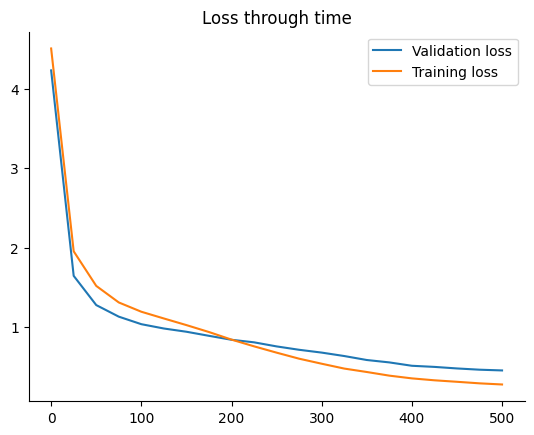
\includegraphics[scale=0.5]{figures/chapter5/loss.png}
    \caption{Gráfica de entrenamiento del modelo, mostrando la pérdida sobre el conjunto de entrenamiento y validación}
    \label{fig:loss}
\end{figure}

\begin{figure}
    \centering
    \begin{subfigure}
        \centering
        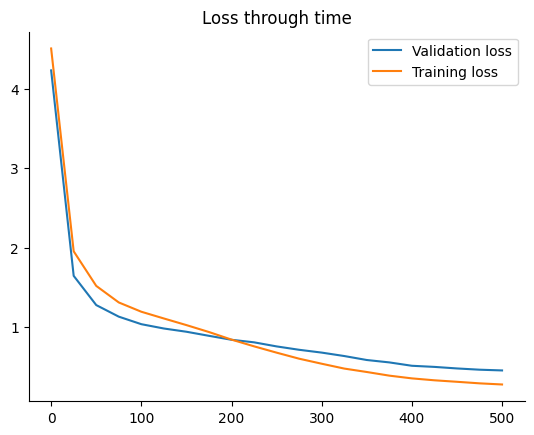
\includegraphics[scale=0.5]{figures/chapter5/loss.png}
        \caption{Gráfica de entrenamiento del modelo, mostrando la pérdida sobre el conjunto de entrenamiento y validación}
        \label{fig:loss}
    \end{subfigure}
    \begin{subfigure}
        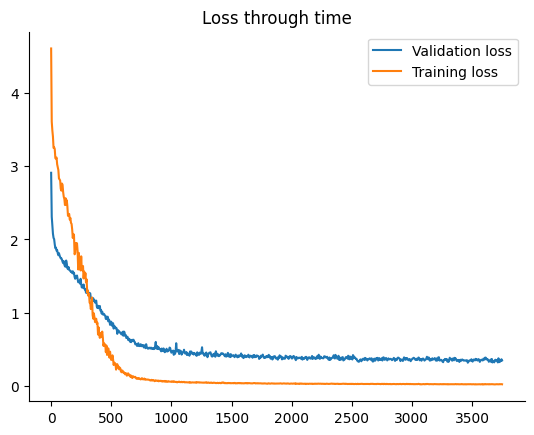
\includegraphics[scale=0.5]{figures/chapter5/loss_big.png}
        \caption{Pérdida sobre el conjunto de entrenamiento y validación a lo largo del entrenamiento. Los valores no son comparables con los de la \cref{fig:loss}, pues la división en símbolos se hace ahora a nivel de palabra, no de caracter. }
        \label{fig:loss_big}
    \end{subfigure}
\end{figure}

\begin{figure}[tb]
    \centering
    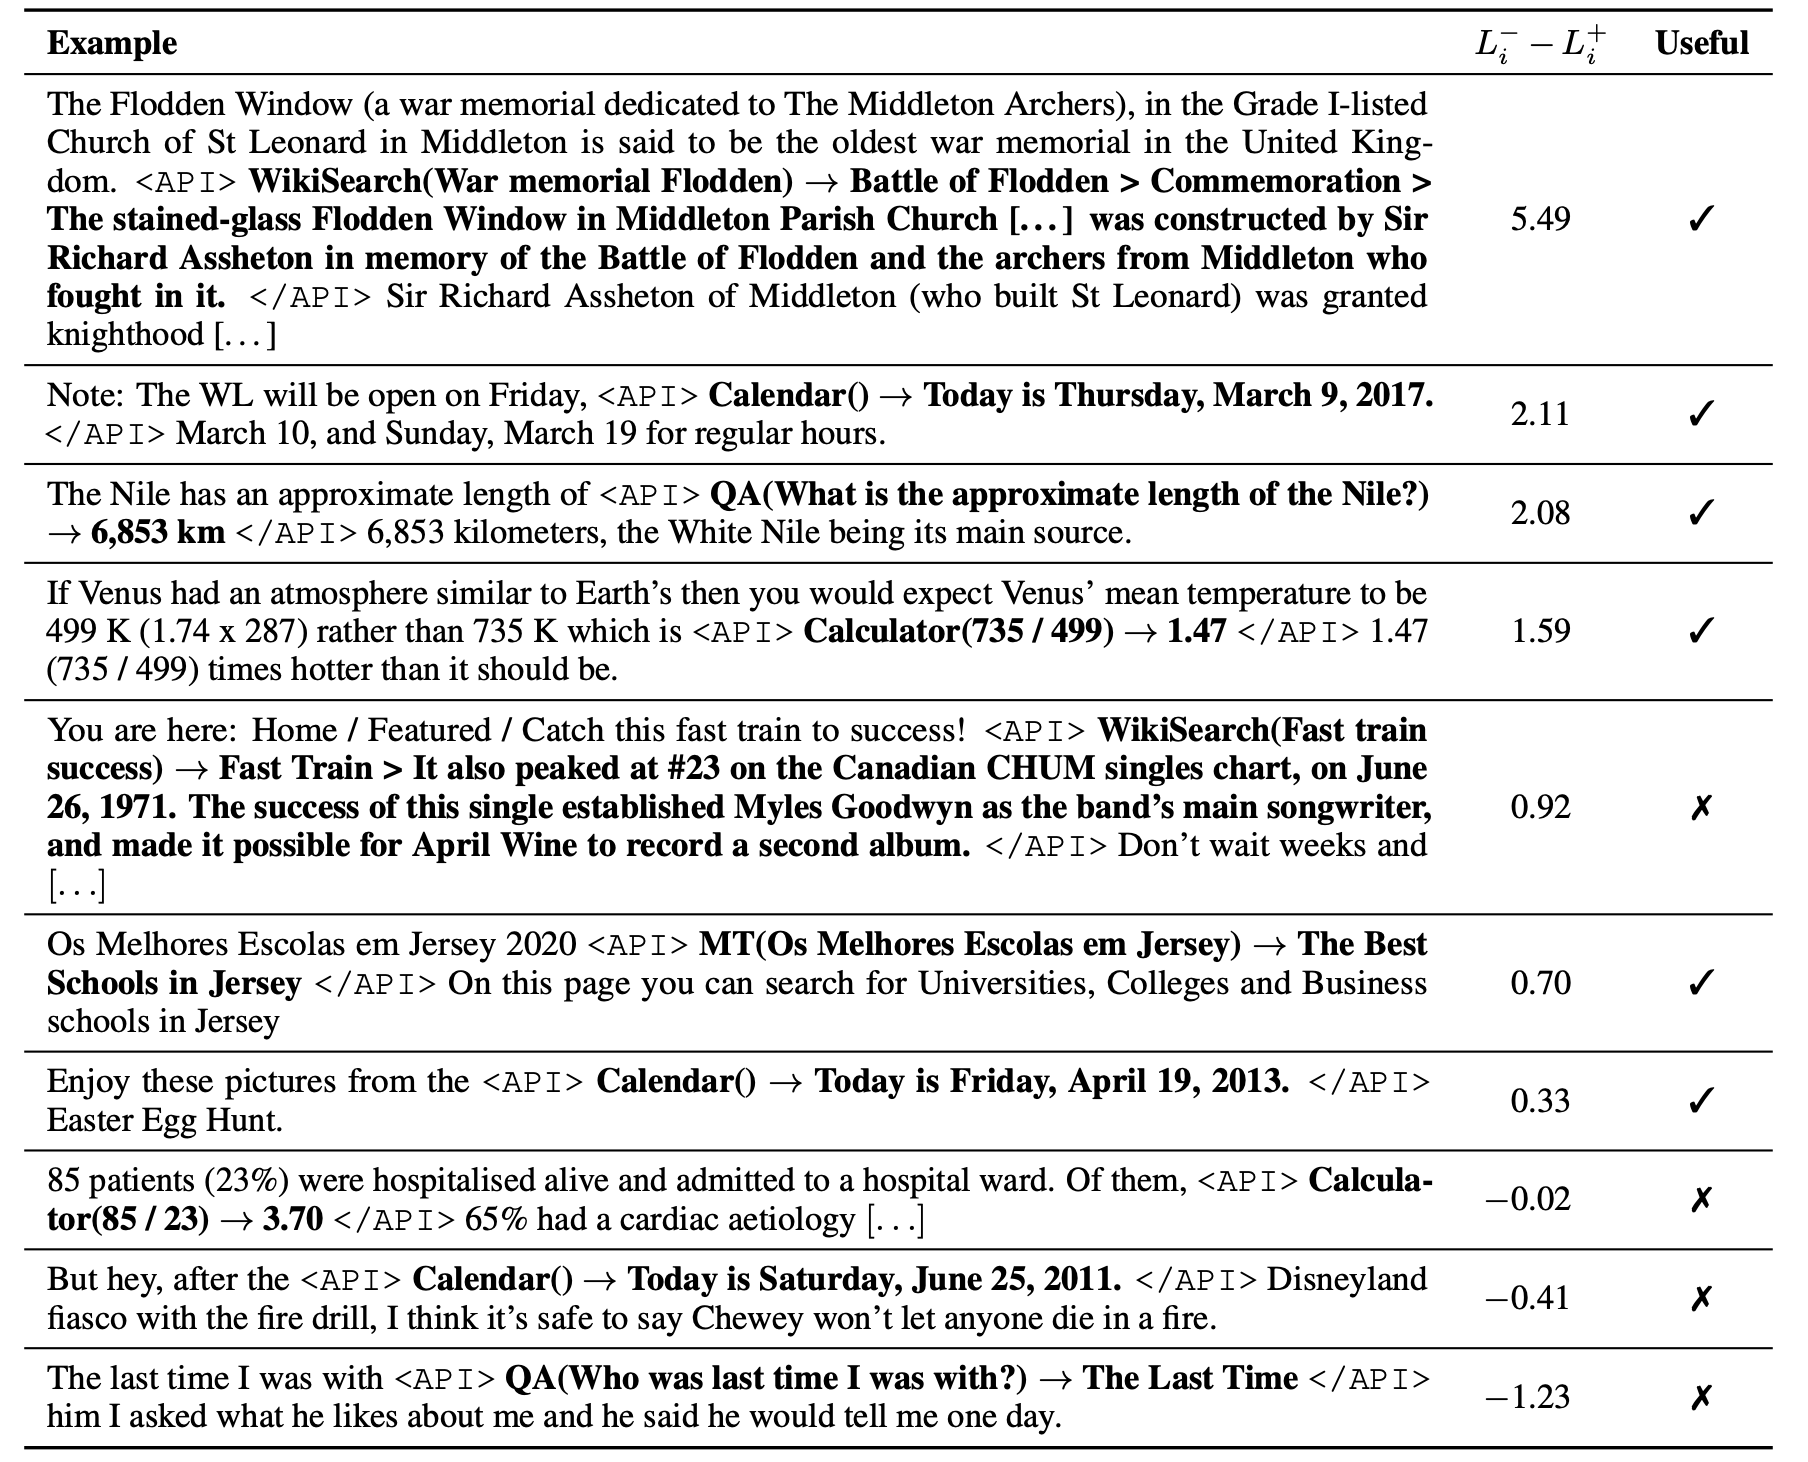
\includegraphics[width=\textwidth]{figures/chapter3/toolformer.png}
    \caption{Ejemplo de llamadas a la API introducidas en la base de datos \cite{schick2023toolformer}. La columna \(L_i^- - L_i^+ \) contiene la diferencia en la evaluación según la entropía cruzada de la respuesta dada por el modelo antes y después de introducir la llamada a la API. \cite{schick2023toolformer}}
    \label{fig:toolformer}
\end{figure}

\begin{figure}[tb]
    \centering
    \begin{subfigure}[b]{0.49\textwidth}
        \centering
        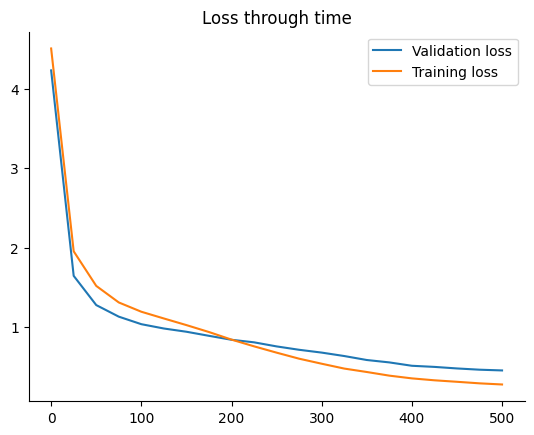
\includegraphics[width=\textwidth]{figures/chapter5/loss.png}
        \caption{Entrenamiento de GPT-1}
        \label{fig:loss}
    \end{subfigure}
    \begin{subfigure}[b]{0.49\textwidth}
        \centering
        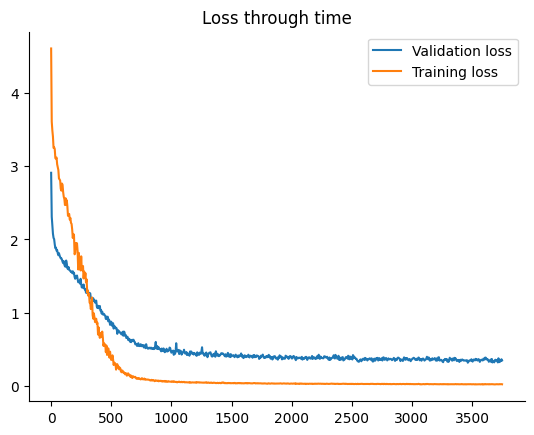
\includegraphics[width=\textwidth]{figures/chapter5/loss_big.png}
        \caption{Entrenamiento de GPT-1}
        \label{fig:loss_big}
    \end{subfigure}
    \caption{Pérdida sobre el conjunto de entrenamiento y validación a lo largo del entrenamiento.}
\end{figure}
